%%%%%%%%%%%%%%%%%%%%%%%%%%%%%%%%%%%%%%%%%%%%%%%%%%%%%%%%%%%%%%%%%%%%
%%%%%%%%%%%%%%%%%%%%%%%%%%%%%%%%%%%%%%%%%%%%%%%%%%%%%%%%%%%%%%%%%%%%
%%                                                                %%
%% Esimerkki opinnäytteen tekemisestä LaTeX:lla                   %%
%% Alkuperäinen versio Luis Costa,  muutokset Perttu Puska        %%
%% Ruotsinkielen tuki lisätty 15092014                            %%
%%                   	                                             %%
%% An example for writting your thesis using LaTeX                %%
%% Original version by Luis Costa,  changes by Perttu Puska       %%
%% Support for Swedish added 15092014                             %%
%%                                                                %%
%% Tähän esimerkkiin kuuluu tiedostot                             %%
%% This example consists of the files                             %%
%%         opinnaytepohja.tex (versio 2.0)                        %%
%%         thesistemplate.tex (versio 2.0) (for text inEnglish)   %%
%%         aaltothesis.cls (versio 2.0)                           %%
%%         kuva1.eps                                              %%
%%         kuva2.eps                                              %%
%%         kuva1.pdf                                              %%
%%         kuva2.pdf                                              %%
%%                                                                %%
%%                                                                %%
%% Kääntäminen joko                                               %%
%% Typeset either with                                            %%
%% latex:                                                         %%
%%             $ latex opinnaytepohja                             %%
%%             $ latex opinnaytepohja                             %%
%%                                                                %%
%%   Tuloksena on tiedosto opinnayte.dvi, joka                    %%
%%   muutetaan ps-muotoon seuraavasti                             %%
%%   Result is the file opinnayte.dvi, which                      %%
%%   is converted to ps format as follows:                        %%
%%                                                                %%
%%             $ dvips opinnaytepohja -o                          %%
%%                                                                %%
%%   ja edelleen pdf-muotoon seuraavasti                          %%
%%   and then to pdf as follows:                                  %%
%%                                                                %%
%%             $ ps2pdf opinnaytepohja.ps                         %%
%%                                                                %%
%% Tai                                                            %%
%% Or                                                             %%
%% pdflatex:                                                      %%
%%             $ pdflatex opinnaytepohja                          %%
%%             $ pdflatex opinnaytepohja                          %%
%%                                                                %%
%%   Tuloksena on tiedosto opinnaytepohja.pdf                     %%
%%   Result is the file opinnaytepohja.pdf                        %%
%%                                                                %%
%% Selittävät kommentit on tässä esimerkissä varustettu           %%
%% %%-merkeillä ja muutokset, joita käyttäjä voi tehdä,           %%
%% on varustettu %-merkeillä                                      %%
%% Explanatory comments in this example begin with                %%
%% the characters %%, and changes that the user can make          %%
%% with the character %                                           %%
%%                                                                %%
%%%%%%%%%%%%%%%%%%%%%%%%%%%%%%%%%%%%%%%%%%%%%%%%%%%%%%%%%%%%%%%%%%%%
%%%%%%%%%%%%%%%%%%%%%%%%%%%%%%%%%%%%%%%%%%%%%%%%%%%%%%%%%%%%%%%%%%%%

%% Käytä toinen näistä:
%% ensimmäinen, jos käytät pdflatexia, joka kääntää tekstin suoraan 
%% pdf-tiedostoksi (kuvat on oltava jpg- tai pdf-tiedostoina)
%% toinen, jos haluat tuottaa ps-tiedostoa (käytä eps-formaattia kuville,
%% alä käytä ps-muotoisia kuvia!)
%%
\documentclass[finnish,12pt,a4paper,pdftex,elec,utf8]{aaltothesis}
%\documentclass[finnish,12pt,a4paper,dvips]{aaltothesis}

%% Kirjoita y.o. \documentclass optioiksi
%% korkeakoulusi näistä: arts, biz, chem, elec, eng, sci
%% editorisi käyttämä merkkikoodaustapa: utf8, latin1
%%

%% Käytä näitä, jos kirjoitat englanniksi. Katso englanninokset tiedostosta
%% thesistemplate.tex.
%%
%% Uncomment one of these, if you write in English:
%% the 1st when using pdflatex, which directly typesets your document in
%% pdf format (use jpg or pdf figures), or
%% the 2nd when producing a ps file (use eps figures, don't use ps figures!).
%\documentclass[english,12pt,a4paper,pdftex,elec,utf8]{aaltothesis}
%\documentclass[english,12pt,a4paper,dvips]{aaltothesis}

%% To the \documentclass above
%% specify your school: arts, biz, chem, elec, eng, sci
%% specify the character encoding scheme used by your editor: utf8, latin1

%%
\usepackage{graphicx}

%% Celsiusmerkille
\usepackage{textcomp}

%% Matematiikan fontteja, symboleja ja muotoiluja lisää, näitä tarvitaan usein 
%%
%% Use this if you write hard core mathematics, these are usually needed
\usepackage{amsfonts,amssymb,amsbsy}

%% Jos et jostain syystä pidä, miten alla oleva hyperref-paketti käyttää
%% fontteja, värejä yms., käytä tämän paketin makroja muuttamaan
%% fonttimäärittelyt. Katso paketin dokumentaatiota. Paketti määrittelee
%% \url-makron, joten ota paketti käyttöön, jos et käytä hyperref-pakettia.
%%
%\usepackage{url}

%% Saat pdf-tiedoston viittaukset ja linkit kuntoon seuraavalla paketilla.
%% Paketti toimii erityisen hyvin pdflatexin kanssa. 
%%
\usepackage{hyperref}
\hypersetup{pdfpagemode=UseNone, pdfstartview=FitH,
  colorlinks=true,urlcolor=red,linkcolor=blue,citecolor=black,
  pdftitle={Default Title, Modify},pdfauthor={Your Name},
  pdfkeywords={Modify keywords}}


%% Kaikki mikä paperille tulostuu, on tämän jälkeen
%%
%% All that is printed on paper starts here
\begin{document}

%% Vain kandityölle: Korjaa seuraavat vastaamaan koulutusohjelmaasi
\degreeprogram{Automaatio- ja systeemitekniikka}
\univdegree{BSc}

%% Oma nimi
\author{Eero Santamala}

%% Opinnäytteen otsikko tulee tähän ja uudelleen englannin- tai 
%% ruostinkielisen abstraktin yhteydessä. Älä tavuta otsikkoa ja
%% vältä liian pitkää otsikkotekstiä. Jos latex ryhmittelee otsikon
%% huonosti, voit joutua pakottamaan rivinvaihdon \\ kontrollimerkillä.
%% Muista että otsikkoja ei tavuteta! 
%% Jos otsikossa on ja-sana, se ei jää rivin viimeiseksi sanaksi 
%% vaan aloittaa uuden rivin.
%% 
\thesistitle{Taajuusmuuttajien käyttö kaivoksissa}

\place{Espoo}
%% Kandidaatintyön päivämäärä on sen esityspäivämäärä! 
%% 

%% For B.Sc. thesis use the date when you present your thesis. 
\date{1.12.2014}

%% Kandidaattiseminaarin vastuuopettaja tai diplomityön valvoja.
%% Huomaa tittelissä "\" -merkki pisteen jälkeen, 
%% ennen välilyöntiä ja seuraavaa merkkijonoa. 
%% Näin tehdään, koska kyseessä ei ole lauseen loppu, jonka jälkeen tulee 
%% hieman pidempi väli vaan halutaan tavallinen väli.
%%
\supervisor{TkT\ Pekka Forsman} %{Prof.\ Pirjo Professori}

%% Kandidaatintyön ohjaaja(t) tai diplomityön ohjaaja(t). Ohjaajia saa
%% olla korkeintaan kaksi.
%% 
%\advisor{Prof.\ Pirjo Professori}
\advisor{TkT\ Pekka Forsman}
%\advisor{DI Tina Tutkija}

%% Aaltologo: syntaksi:
%% \uselogo{aaltoRed|aaltoBlue|aaltoYellow|aaltoGray|aaltoGrayScale}{?|!|''}
%% Logon kieli on sama kuin dokumentin kieli
%%
\uselogo{aaltoRed}{''}

%% Tehdään kansilehti
%%
\makecoverpage


%% Suomenkielinen tiivistelmä
%% Kaikki tiivistelmässä tarvittava tieto (nimesi, työnnimi, jne.) käytetään
%% niin kuin se on yllä määritelty.
%% Tiivistelmän avainsanat
%%
\keywords{Avainsanoiksi valitaan kirjoituksen sisältöä keskeisesti kuvaavia
käsitteitä}
%% Tiivistelmän tekstiosa
\begin{abstractpage}[finnish]
 Tiivistelmä suomeksi.
\end{abstractpage}

%% Pakotetaan uusi sivu varmuuden vuoksi, jotta 
%% mahdollinen suomenkielinen ja englanninkielinen tiivistelmä
%% eivät tule vahingossakaan samalle sivulle
%%
\newpage

\mysection{Esipuhe}

Kiitos ABB ja sillee jee.\\

\vspace{5cm}
Otaniemi, 1.12.2014

\vspace{5mm}
{\hfill Eero H.\ Santamala \hspace{1cm}}

%% Pakotetaan varmuuden vuoksi esipuheen jälkeinen osa
%% alkamaan uudelta sivulta
\newpage


%% Sisällysluettelo
\thesistableofcontents


%% Symbolit ja lyhenteet
\mysection{Symbolit ja lyhenteet}

\subsection*{Symbolit}


\subsection*{Operaattorit}



\subsection*{Lyhenteet}

\begin{tabular}{ll}
AC         & vaihtovirta \\
DC         & tasavirta \\
IEC	       & International Electrotechnical commission \\
NEMA       & National Electrical Manufacturers Association \\
\end{tabular}


%% Sivulaskurin viilausta opinnäytteen vaatimusten mukaan:
%% Aloitetaan sivunumerointi arabialaisilla numeroilla (ja jätetään
%% leipätekstin ensimmäinen sivu tyhjäksi, 
%% ks. alla \thispagestyle{empty}).
%% Pakotetaan lisäksi ensimmäinen varsinainen tekstisivu alkamaan 
%% uudelta sivulta clearpage-komennolla. 
%% clearpage on melkein samanlainen kuin newpage, mutta 
%% flushaa myös LaTeX:n floatit 
%% 
\cleardoublepage
\storeinipagenumber
\pagenumbering{arabic}
\setcounter{page}{1}


%% Leipäteksti alkaa
%%
\section{Johdanto}

%% Ensimmäinen sivu tyhjäksi
%% 
\thispagestyle{empty}
Taajuusmuuttajia käytetään yhä enenemässä määrin vaihtovirtasähkömoottoreiden ohjaukseen kaikilla teollisuudenaloilla ja erityisesti kaivosteollisuudessa \cite[s. 262]{Hakapää}. %%s. 262: taajuusmuuttajat 
Erilaiset käyttöympäristöt ja -sovellukset vaikuttavat taajuusmuuttajalta vaadittuun toiminallisuuteen ja fyysisiin ominaisuuksiin. Käyttökohteesta riippuvat ominaisuudet luovat taajuusmuuttajavalmistajille näin tarpeen kartoittaa eri teollisuudenalojen erityisvaatimuksia, jotta tuotteet pystytään kehittämään vastaamaan asiakkaiden tarpeita mahdollisimman hyvin. 
\\\\
Tämän työn tarkoituksena on tarkastella kaivosteollisuuden asettamia vaatimuksia ja tarpeita taajuusmuuttajan toiminnallisuudelle ja kestävyydelle sekä kartoittaa millaisia eri sovelluksia taajuusmuuttajille kaivostoiminnassa esiintyy. Tämän työn yhteydessä kaivosteollisuudella tarkoitetaan kaivosta ja sen välittömässä läheisyydessä tapahtuvaa malmin siirtoa ja käsittelyä ja tarkastelu keskittyy yksinomaan siihen. Mineraalien jatkokäsittely kaivosalueen ulkopuolella muistuttaa jo tavanomaista prosessiteollisuutta, eikä siksi ole tämän työn kannalta mielenkiintoista.
\\\\
Yleisin taajuusmuuttajan sijoituspaikka on sisätiloissa esimerkiksi tuotantolaitoksen sähköhuoneessa. Tällöin ympäristöolosuhteet saadaan pysymään hyvin tasaisina ja taajuusmuuttajan toiminnalle edullisina. Lämpötila- tai kosteusvaihteluita ei ilmastointijärjestelmän ansiosta juuri ole ja huoneen ilma on suodatettu pienpartikkeleista jo ennen sen pääsyä kosketuksiin taajuusmuuttajan kanssa. Kaivosteollisuudessa vastaavan tasaisen käyttöympäristön järjestäminen voi olla epäkäytännöllistä tai taloudellisesti kannattamatonta, jolloin taajuusmuuttajalta itseltään edellytetään kestävyyttä ja toimintavarmuutta vaativissakin käyttöympäristöissä. Myös kaivoksen sähköverkko asettaa taajuusmuuttajalle omat vaatimuksensa.
\\\\
Työn alussa selvitetään kaivosympäristön erityisvaatimukset lähtien liikkeelle ympäristöolosuhteista. Osan tarkoituksena on luoda selvä kuva kaivoksen asettamista vaatimuksista siellä käytettävälle laitteistolle jotta voidaan ymmärtää mitä taajuusmuuttajilta vaaditaan. Tarkastelun alla ovat lisäksi standardit, jotka kaivoteollisuuden laitteita koskevat.
\\\\
Seuraavassa osassa esitetään millaista toiminnallisuutta taajuusmuuttajien sisäisillä logiikkapiireillä voidaan toteuttaa ja miten niitä voidaan hyödyntää kaivosteollisuuden sovelluksissa. Viimeisessä osassa esitetään taajuusmuuttajien käyttökohteita kaivoksissa lähtien liikkeelle taajuusmuuttajien tyypillisestä sijoittelusta sekä tyypillisistä teho- ja jänniteluokista. Sovellukset-osio käy läpi suurimmat teollisuudenalan sähkövoimaa käyttävät sovellukset ja kertoo millaisia taajuusmuuttajaratkaisuja niissä käytetään ja mitä hyötyjä taajuusmuuttajien käyttö niissä tuo verrattuna perinteisiin ohjausratkaisuihin.
\\\\
Työssä on oleellista taajuusmuuttajien hyödyntäminen ja niistä saatava lisäarvo kaivosteollisuuden asiakkaan näkökulmasta. Se keskittyy sovelluksiin ja niiden vaatimuksiin eikä niinkään taajuusmuuttajan sisäisiin ratkaisuihin näiden hyötyjen aikaansaamiseksi. Työ esittää alan olemassa olevat taajuusmuuttajaratkaisut ja pohtii mitä lisäarvoa taajuusmuuttajilla voitaisiin vielä saavuttaa.

\clearpage
\section{Kaivosympäristön vaatimukset taajuusmuuttajalle}

\subsection{Ympäristöolosuhteet}
Kuten todettu, kaivosympäristö on sähkölaitteille toimintaympäristönä erittäin rasittava \cite[s. 251]{Hakapää}. %% "Kaivoksen olosuhteet ovat raskaimpia, missä sähkölaitteita käyetetään." <-- sitaatiksi?
Sähkölaitteille kaivoksissa rasitusta aiheuttavia tekijöitä ovat
\begin{itemize}
	\item[--] Lämpötila
	\item[--] Kosteus
	\item[--] Ilman epäpuhtaudet
	\item[--] Mekaaniset rasitukset
\end{itemize}
Suurin ympäristön aiheuttama vaara taajuusmuuttajien toiminnalle on ylikuumeneminen ja elektronisten komponenttien vaurioituminen kosteuden, ilman  epäpuhtauksien, mekaanisten iskujen tai tärinän seurauksena. Jotta taajuusmuuttajan luotettava toiminta voidaan taata, täytyy taajuusmuuttajan koteloinnin olla soveltuva käyttöympäristöönsä. Lähes kaikki taajuusmuuttajavalmistajat valmistavatkin taajuusmuuttajia eri suojausluokissa vastaamaan sovellusten vaatimuksia.
\\\\
Euroopassa yleisesti käytössä oleva luokitus sähkölaiteen vesi- ja pölytiiveydelle on kansainvälisen sähköalan standardointitoimiston IEC:n IP-luokitus. Luokitus on kaksiosainen lähtien täysin suojaamattomasta IP00-luokasta ja päätyen täysin vesi- ja pölytiiviiseen IP69-luokitukseen [LIITE 1 TÄHÄN]. Pohjois-Amerikassa on käytössä vastaava NEMA-tiiveysluokitus.
\\\\
Markkinoilla olevat taajuusmuuttajat ulottuvat suojaamattomista IP00-laitteista aina lähes vesitiiviisiin IP66-laitteisiin. IP00 taajuusmuuttajat asennetaan poikkeuksetta ulkoisiin koteloihin, jännitteellisten komponenttien ollessa täysin esillä. IP21 on yleinen käytössä oleva luokka taajuusmuuttajille, jotka tulevat kuivaan tilaan esimerkiksi tehtaan sisälle. Märkiin tai muuten erityistä suojausta vaativiin sovelluksiin tarkoitetut IP66 laitteet kestävät suoran painevesiruiskun kaikista suunnista ja ovat täysin pölysuojattuja. Suuremman suojausluokituksen omaavat laitteet ovat luonnollisesti fyysisesti suurempia ja mekaanisesti haastavampia rakentaa. LÄHDE?
\\\\
Seuraavissa kappaleissa eritellään eri ympäristötekijöiden merkitsevyys kaivosympäristössä. Tarkastelun alla ovat myös tavat mitä vaikutuksia näillä olosuhteilla on taajuusmuuttajien toiminnalle sekä miten nämä asiat on otettu huomioon taajuusmuuttajien suunnittelussa. Käsittely koskee pääosin maanalaisia kaivoksia avolouhosten olosuhteiden ollessa tavallista ulkoilmakäyttöä vastaavat. %%such metatext

\subsubsection{Lämpö}
%%-Kaivosten lämpötilat
%%-Laitteiden käyttölämpötilat, derating
%%-Jäähdytysratkaisut(neste,kanava,perinteinen,cold plate,...)
Maanalaisissa kaivoksissa lämpöolosuhteet eroavat huomattavasti maanpäällisistä. Kaivoksessa lämpöä aiheuttaa itse kallioperän lämpö, ilman puristuminen, lämpimät pohjavesivuodot, koneet, valaistus ja räjäytykset.
\\\\
Etenkin syvissä kaivoksissa kallioperän lämpö on suurimpia kaivoksen sisäilman lämmittäjiä. Kallioperän lämpötila kasvaa syvemmälle mentäessä noin 25-30\textdegree C/km, joten jo kilometrin syvyisessä kaivoksessa lämpötila voi yltää 30-40\textdegree C riippuen paikallisesta ilmastosta \cite[s. 62]{maanlampo}. %% s.62: maan lämpeneminen/km 
Esimerkkinä todettakoon Suomen syvin metallikaivos Pyhäsalmella on 1400 metriä syvä, jolloin lämpötila ilman ilmanvaihtoa kohoaa yli kolmeenkymmeneen asteeseen.
\\\\
Hyvin suunnitellussa kaivoksessa kuitenkaan harvoin on ongelmana, että kaivoksen sisälämpötila olisi liian korkea laitteiden toiminnalle. Olennaista on, että lämpö pystytään johtamaan ulos sitä tuottavista laitteista ja ilmaa lämmittävästä kallioperästä jotta lämpötila pysyy koneille ja henkilöstölle edullisena. Ilmanvaihtojärjestelmän suunnittelun tärkeys tulee tässä vahvasti esille.
\\\\
Taajuusmuuttajat ovat hyvin energiatehokkaita laitteita siirtäen noin 98\% vastaanottamastaan energiasta moottorille\cite{ABBinmining}. Energiasta 2\% kuitenkin muuttuu taajuusmuuttajan sisäisenä häviönä lämpöenergiaksi. Tämä tarkoittaa esimerkiksi 500kW taajuusmuuttajan vaativan noin 10kW jäähdytystehon toimiakseen jatkuvasti. Tämä lämpöenergia poistetaan taajuusmuuttajasta ilma- tai nestejäähdytyksen avulla ympäristöön.
 
%%derating ja muut suojat????

%%Taajuusmuuttajien ratkaisut flange ym ilmastointitavat?

%%flange vasta partikkeleihin???



\subsubsection{Kosteus}
%%-Kaivosten kosteus, sumu, kaapelit vesitiiviitä
%%-Laitteiden kosteuskestävyys?
%%-IP ja - NEMA-luokitukset?
Kosteus voidaan jakaa kahteen luokkaan: ilmankosteuteen ja nestemäiseen veteen. Suurimman uhan sähkölaitteen toiminnalle aiheuttaa nestemäinen vesi, jota kondensoituu kosteasta ilmasta. Kaivoksissa suhteellinen ilmankosteus saattaa nousta hyvinkin koreaksi suljetun tilan sitoessa kostean ilmamassan.  Syvimmissä kaivoksissa voidaan saavuttaa jopa yli 95\% suhteellinen ilmankosteus \cite{manchao}. Kondensoituvan veden lisäksi kaivoksissa täytyy ottaa huomion myös katosta mahdollisesti tihkuva vesi.
\\\\
Kaivoksen tekniikkaa suunniteltaessa on otettava huomioon sähkölaitteiden kosteudensieto ja sijoitettava laitteet joko eristettyyn sähkötilaan tai hankkia ne riittävällä suojausluokituksella varustettuna. Ilmajäähdytteisten laitteiden haasteena on yleisesti niiden pienempi IP-luokitus, mikä sallii veden kondensoitumisen laitteen sisälle\cite{Pallasmaa}. Vesijäähdytys tarjoaa yleisesti paremman tiiveysluokituksen, sillä laitetta viilentää ilman sijasta suljettu nestejärjestelmä. Kaivoksen tilapäisen luonteen vuoksi nestejärjestelmät voivat kuitenkin osoittautua epäkannattaviksi.
\\\\
Jotta myös ilmajäähdytteisiä laitteita pystytään käyttämään vaativissa olosuhteissa täytyy korkeamman suojausluokan laitteissa jäähdytysilma johtaa laitteen läpi sen pääsemättä kosketuksiin elektroniikan kanssa. Tämä on usein toteutettu jakamalla laite sisäisesti kahteen osaan: kosteudelle herkän elektroniikan sisältävään osioon ja jäähdytysosioon, jossa jäähdytyselementti  sijaitsee.  Lämpö johtuu komponenteista jäähdytyselementin säleikköön, josta se johtuu säleikön läpi kulkevaan ilmaan. Ilma kierrätetään laitteen läpi tuulettimilla, joiden täytyy kestää ympäristön olosuhteet. Tuuletin onkin yksi ilmajäähdytteisen taajuusmuuttajan herkimmin hajoavia komponentteja. Kuva~\ref{fig:IP55} esittää IP55 luokitellun taajuusmuuttajan, jossa jäähdytysilma ohjataan jäähdytyselementin kautta sen pääsemättä kosketuksiin elektroniikan kanssa. \cite{Muttilainen}.
\\
\begin{figure}[h]
	\begin{center}
	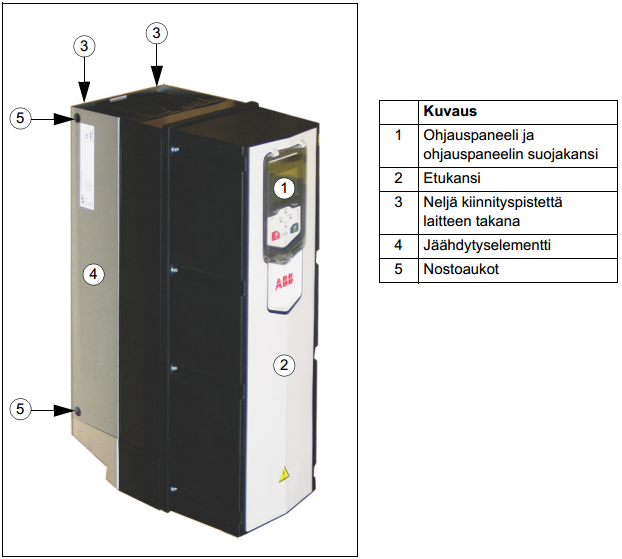
\includegraphics{IP55}
	\end{center}
	\caption{ACS880-01 taajuusmuuttaja IP55-koteloinnilla
		\cite[s.28]{880hwman}}
	\label{fig:IP55}
\end{figure}

Toinen mahdollisuus on sijoittaa jäähdytyselementti laitteen ulkopuolelle, jolloin yleisesti puhutaan niin sanotusta laippa-asennuksesta (flange-installation). [Lähde] Tällä tekniikalla taajuusmuuttaja pysytään upottamaan ulkoiseen koteloon ja kierrättämään jäähdytysilma kotelon ulkopuolella esimerkiksi tuuletuskanavassa. Tämä eristää taajuusmuuttajan täysin tuuletusilmasta ja sallii tehokkaan lämmön poistamisen tuuletuskanavan välityksellä.
\\\\
Kaivoksen kiinteissä asennuksissa on mahdollista rakentaa myös kokonaisia kosteuden- ja pölynkestäviä sähköhuoneita, joissa pystytään käyttämään normaalin IP21 tai IP20 tiiveysluokituksen omaavia sähkölaitteita \cite[s.253]{Hakapää}. Taajuusmuuttajien sijoittelu näihin pysyviin rakennelmiin voi kuitenkin olla kannattamatonta moottorikaapelien pituuksien kasvaessa kohtuuttoman pitkiksi.





%%Pallasmaa Aaro selvitä dippatyö: ulkokäyyttöön suunnitellun tehoelektroniikkalaitteen konseptisuunnittelu.

%%ACS880-01 HW manual, kuvat tuuletuskanavista ja laitteesta!!
%%ACS880-01 Flange-manual lähteeksi?

%%Kysy petriltä EMC-häiriöistä!
%% flangen ip-luokka?

%%ota mallia dippa: Lifetime and reliabilty of .... fan	

\subsubsection{Pienpartikkelit}
%%-Pöly\\
%%-Kemikaalit\\
%%-Syövyttävyys\\
%%-Elektroniikan eristys (flange)
Kaivoksen ilmassa on kosteuden lisäksi pölyä ja muita kemikaaleja, joita muodostuu työkoneiden ja räjäytysten seurauksena. 

MItä kaikkea kaivoksissa pölyää : \cite{Howard}


%-kiviainesta
%-räjähteitä
%-Mitä aiheuttaa?
%-tuulettimet tukkeutuu
%-vesi + paska = korroosio
%-elektroniikan yhteydessä läpilyöntejä

\subsubsection{Mekaaniset rasitukset}
-kuljetus,asennus\\
-Tärinä (murskaimet yms. Liikkuvat laitteet?)


\subsection{Kaivoksen sähköverkko}
Kaivoksen sähköverkko (EMC häiriöt)\\
-jännite,laajuus, häiriönsieto, EMC\\
-kuristimien/filttereiden tarpeellisuus

\subsection{Käyttöikä ja luotettavuus}
-kaivoksen ikä? Sama laite koko elinkaaren?\\
-Esim tuuletusjärjestelmän luotettavuus ensisijaisen tärkeää?\\
-Redundanttius?\\
-Virran katkeaminen? varavoimalähteet?

\subsection{Kaivosteollisuuden standardit}
-ex-luoitus: Räjähdysherkkä tila?\\
-mitä muita?




\clearpage
%%--------------------------TOIMINNALLISUUS-----------------------------------
\section{Taajuusmuuttajien toiminnallisuus}
Milaisia toimintoja taajuusmuuttajista löytyy?\\
Tamujen kehitys

\subsection{Toimintasyklit}
-Millaisia tamuista löytyy (rampit, pid, vektoriohjaus, ABB:n DTC momenttiojaus,)\\
-Vaihtoehtoiset ohjaustavat (softstartterit yms), Hyödyt? (verkon heilahdukset, energiansäästö, tarkemmat prosessit)\\


--Nää ehkä sovellukset osioon?----\\
-Murskaimet \cite{Hulthen}\\
-Kuljettimet (ramppikäynnistys? kuorman mukaan säätyminen?)\\
-Multidrives? ACS800 OPM (open pit mine) control program?


\subsection{Turvallisuustoiminnot}
-turvallisuus tärkeää, kaivokset vaarallisia jne.\\
-STO, miten voisi hyödyntää?\\
-Profisafe yms.

\subsection{Mittaukset}
-Kuljettimet, määrän mittaus kuormasta ja nopeudesta?
-MItä muuta (malmivirtojen mallinnus)

\subsection{Ohjaus ja -valvontajärjestelmät}
-Keskitetty automaatiojärjestelmä?
-Kenttäväylät?
-
\subsection{Verkkoon jarruttavat taajuusmuuttajat}
-miten käytännössä toimii\\
-Missä voidaan hyödyntää? (hissit, alamäkeen jarrutus, dumppitrukkien sähköraidejärjestelmä, yms.)

\clearpage

\section{Taajuusmuuttajien sovellukset kaivoksissa}

\subsection{Kokoluokat ja sijoittelu}
-Teho- ja jänniteluokat (kuvia!)\\
-Seinä,lattia,floorstanding\\
-Asennuspaikat\\
-fyysinen koko?\\
-Hyvät/huonot puolet\\
-kaapelien pituus, EMC

\subsection{Sovellukset}
\subsubsection{Kaivinkoneet}
-mitä erilaisia? (jäätävän isot osana sähköverkkoa vs pienet)\\
-Multidrive ohjaamaan kaikkea?


\subsubsection{Liukuhihnat ja kuljettimet}
-Millaisia erilaisia? (liukuhihnat,ruuvit,nostimet,yms.)\\
-Nykyratkaisut?\\
-Miten tamuja hyödynnetään? edut perinteiseen verrattuna?

\subsubsection{Murskaimet}
-Millaisia? kuinka isoja?\\
-Toimintasyklit? \cite{Hulthen}\\
-Automaation taso?

\subsubsection{Hissit}
-Henkilöhissit, junat, kärryt. Millä ihmiset liikkuu?

\subsubsection{Tuulettimet ja ilmanvaihto}
-Kaivoksen tuulettaminen!\\
-Miten tehty?\\
-Ohjaus, valvonta?\\
-Varajärjestelmät?

\subsubsection{Pumput}
-mutapumput, vesipumput.\\
-puhdistus\\
-mittaukset

\subsubsection{Paineilman tuottaminen?}
Paljon sähköä kuluttava?\\
Mihin käytetään kaivoksissa?\\
Miten tamuja voidaan hyödyntää?
%%fi.opasnet.org./fi/Metallimalmikaivostoiminnan_elinkaari

\clearpage

\section{Yhteenveto}
-Energiansäästö\\
-Kustannukset\\
-Tarkemmat prosessit\\
-Tulevaisuus?

-->profit

%\section{Summary} 

\clearpage

%% Lähdeluettelo
\thesisbibliography
\begin{thebibliography}{99}
	
\bibitem{maanlampo}Fridleifsson, Ingvar B., Bertani, Ruggero, Huenges, Ernst, Lund, John W., Ragnarsson, Arni ja Rybach, Ladislaus. \textit{The possible role and contribution of geothermal energy to the mitigation of climate change.} IPCC Scoping Meeting on Renewable Energy Sources. Luebeck, Germany, 2008, Saatavissa: \url{http://www.ipcc.ch/pdf/supporting-material/proc-renewables-lubeck.pdf}

\bibitem{Hakapää}Hakapää,\ A. ja Lappalainen,\ P. \textit{Kaivos- ja louhintatekniikka.} 2.\ painos. Helsinki, Vammalan kirjapaino Oy, 2007.

\bibitem{IP}IEC 60529. \textit{Degrees of protection provided by enclosures (IP Code).} Versio 2.1, Geneve, Sveitsi, International Electrotechnical Commission, 2001.

\bibitem{Rumpunen}Rumpunen, A. \textit{Tuulivoiman vaatimukset taajuusmuuttajalle.} Kandidaatintyö. Aalto-yliopisto. 
Insinööritieteiden korkeakoulu. Espoo. 2012.

\bibitem{ABBtechnicalguide}ABB Drives \textit{Technical guide book}, 2008.

\bibitem{Lukkarinen}Lukkarinen T. \textit{Mineraalitekniikka Osa 1 Mineraalien hienonnus.} Hki: Insinööritieto Oy, 1984.

\bibitem{Anttila}Anttila A. \textit{Kaivosten tuuletusilman energiatehokas lämmitys Suomessa.} Kandidaatintyö. Aalto-yliopisto. Insinööritieteiden korkeakoulu. Espoo. 2014.

\bibitem{Muttilainen}Muttilainen, A. \textit{Lifetime and Reliability of a Frequency Converter’s Fan.} Diplomityö. Aalto-yliopisto. Sähkötekniikan korkeakoulu. Espoo. 2013

\bibitem{Karlsson}Karlsson, S. \textit{Murskaintyyppien ominaisuuksien vertailu}. Kandidaatintyö. Aalto-yliopisto. Insinööritieteiden korkeakoulu. Espoo. 2011.

\bibitem{Hulthen}Erik Hulthén, C. Evertsson, M. \textit{Real-time algorithm for cone crusher control with two variables}. Minerals Engineering.  24. Painos. Numero 9. Elokuu 2011. s. 987-994. Saatavissa: \url{http://dx.doi.org/10.1016/j.mineng.2011.04.007}.

\bibitem{Pyhäsalmi}CUPP, \textit{Pyhäsalmen kaivos.} Verkkodokumentti. Päivitetty 26.3.2013. Viitattu 6.10.2014. Saatavissa: \url{http://www.cupp.fi/index.php?option=com_content&view=article&id=3&Itemid=41&lang=fi	}

\bibitem{ABBinmining}ABB Oy. \textit{ABB drives in mining}. Päivitetty 2012. Viitattu 6.10.2014. Saatavissa: \url{http://www05.abb.com/global/scot/scot216.nsf/veritydisplay/2205e72865c2c747c1257a620026d001/$file/Mining%20brochure_EN_lowres.pdf}

\bibitem{manchao}Man-chao, H. \textit{Application of HEMS cooling technology in deep mine heat hazard control}. Mining Science and Technology (China). 19. Painos, Numero 3. Toukokuu 2009. S. 269-275. Saatavissa: \url{http://dx.doi.org/10.1016/S1674-5264(09)60051-X}.

\bibitem{880hwman}ABB Oy. 2012. \textit{Laiteopas, ACS880-01-taajuusmuuttajat, Rev E}. Saatavissa: \url{http://www05.abb.com/global/scot/scot201.nsf/veritydisplay/71ce8071e2a7ae2bc1257bd70046ade1/$file/FI_ACS880-01_0_55to250kW_HW_E_plus_update_notice_screen.pdf}. Päivitetty 29.6.2012. Viitattu 9.10.2014.

\bibitem{Pallasmaa}Pallasmaa, A. \textit{Ulkokäyttöön Tarkoitetun Tehoelektroniikkalaitteen Konseptisuunnittelu}. Diplomityö. Teknillinen korkeakoulu. Espoo. 2009.

\bibitem{Howard}Hartman, H. Mutmansky, J. Ramani, R. Wang, Y. \textit{Mine Venilation and Air Conditioning}. New York, Yhdysvallat. John Wiley & Sons Inc. 1997.




\end{thebibliography}



%% Liitteet
\clearpage

\thesisappendix
\section{Liite 1\label{LiiteA}}
IP-luokat taulukossa

\end{document}
